\chapter{Использование нейронных сетей в задачах регрессии}

\section{Задача регрессии в машинном обучении}
С помощью обученных моделей нейронных сетей можно решать обширный класс задач. Регрессия — нахождение максимально простой и близкой к исходным данным функции, используя механизм минимизации потерь. Потери в данном контексте — ошибки, вычисленные различными метриками.
\subsection{Метрики и параметры качества}
Различие метрик и функций потерь (параметров качества) состоит в том, что метрики используются при оценке качества работы модели, а функции потерь используется непосредственно при обучении, но математические основы у них одни.\cite{31, 32}
Для задач регрессии выделяют три основные функции потерь:
\begin{enumerate}
    \item [1)] средний квадрат отклонения, основанный на $L_{2}$ норме;
    \item [2)] среднее абсолютное отклонение, основанный на $L_{1}$ норме;
    \item [3)] средний квадрат логарифмического отклонения, который вычисляется по следующей формуле \ref{e:5}:
    \begin{equation}\label{e:5}
    E = \frac{1}{N}\sum (log(x_{n}+1)-log(y_{n} + 1))^2.
    \end{equation}
\end{enumerate}
При использовании алгоритма обратного распространения ошибки функции потерь определяют длину шага для метода градиентного спуска. Средний квадрат ошибок выдает большой шаг по градиенту при наличии больших, но даже редких ошибок из-за квадратной зависимости $n^2$, также у этого критерия качества множество локальных минимумов, из-за чего его стоит использовать при отсутствии сильных отклонений. Средний модуль отклонения не так чуствителен к редким значительным ошибкам. Средний квадрат логарифмического отклонения используется для обучения с большими и редкими ошибками, т.к. они не сильно увеличивают шаг из-за логарифмической зависимости. Так же есть функция среднеквадратичного отклонения, он приводит средний квадрат отколнения в линейную зависимость и функция среднего абсолютного процента ошибки, с ее помощью можно посчитать процент ошибки \ref{e:6}:
\begin{equation} \label{e:6}
    E = 100\% \cdot \frac{1}{N}\sum \frac{|x_{n}-y_{n}|}{max(|Y|, \epsilon)}.
\end{equation}
Она нужна, чтобы не брать во внимание конкретные значения и видеть долю возможной ошибки.
\cite{20}.
\subsection{Линейная и нелинейная модель регрессии}
Линейная модель регрессии (рисунок \ref{fig:2}) используется для установки линейной связи между одной или несколькими независимыми переменными и числовым результатом или зависимой переменной. Она используется для прогнозирования, экстраполяции и упрощения сложных зависимостей.
\cite{17,25}.

\begin{figure}[ht] 
  \center
  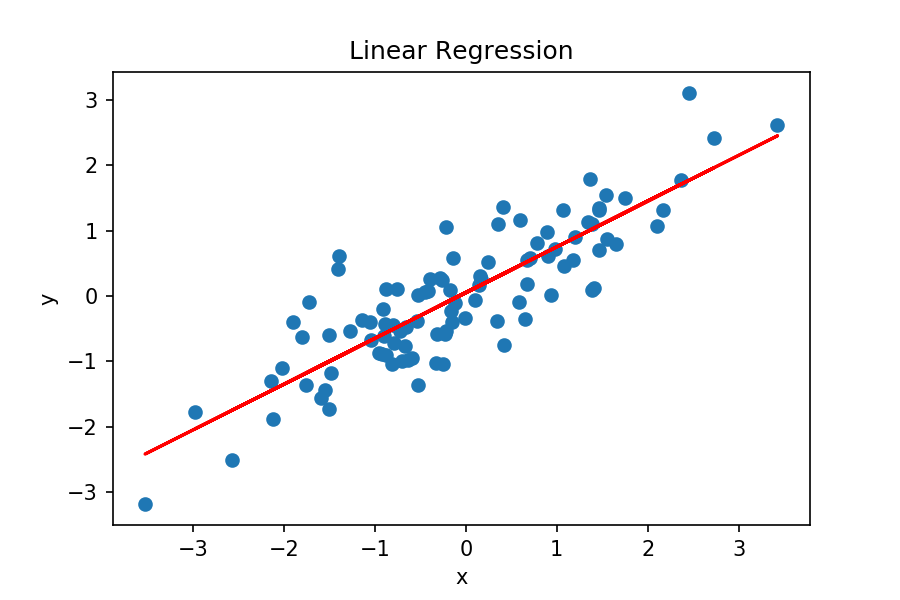
\includegraphics [scale=0.5] {img/linear_reg.png}
  \caption{Пример линейной регрессии} 
  \label{fig:2}  
\end{figure}
\newpage
Нелинейная регрессия (рисунок \ref{fig:3})  — это тип полиномиальной регрессии, использующийся как метод моделирования нелинейной зависимости между зависимыми и независимыми переменными. Она дает более точные прогнозы, которые не являются линейной аппроксимацией. Она работает лучше линейной регрессии в задачах, где прогнозируемая функция является достаточно сложной, в связи с чем линейная регрессия не дает достаточно точных результатов.\cite{29, 30}


\begin{figure}[ht] 
  \center
  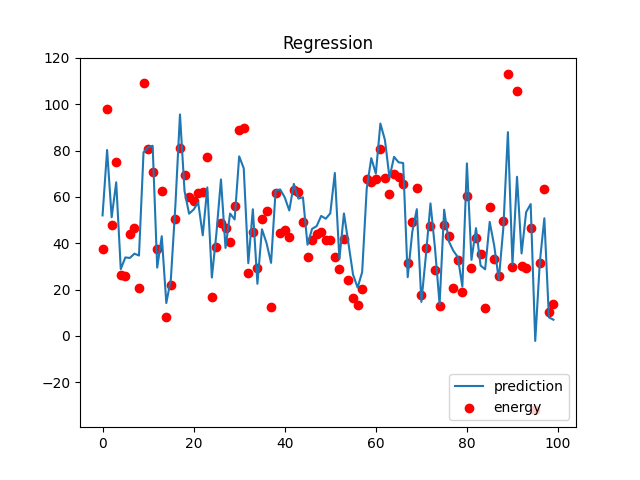
\includegraphics [scale=0.9] {img/non_linear_reg.png}
  \caption{Пример нелинейной регрессии} 
  \label{fig:3}  
\end{figure}
\newpage
\section{Архитектура и процесс обучения нейронной сети}
В качестве задачи регрессии было взято предсказание молекулярных свойств, а именно энергии основного состояния. Для решения задач регрессии используются полносвязные нейронные сети. На выходе у такой сети обычно 1 нейрон, а функция активации этого нейрона должна быть линейной. В качестве признаков, по которым будет строится прогноз будут выступать структуры молекул, а именно заряды ядер атомов и их взаимное расположение. Эти данные необходимо преобразовать в вектор признаков. В научной литературе существует несколько подходов \cite{26, 27, 28}, один из которых заключается в использовании кулоновской матрицы для данной молекулы, которая определяется как \ref{e:7}:
\begin{equation} \label{e:7}
    C_{IJ} = \frac{Z_I Z_J}{\vert R_I - R_J \vert}, ({\rm I \neq J});
    C_{IJ} = Z_I^{2.4}, (I=J),
\end{equation}
где Z — заряд ядра атома молекулы.

Данная матрица симметрична относительно главной диагонали, поэтому в вектор признаков будут записаны только значения самой диагонали и выше нее. Эти данные будут поданы на вход полносвязной нейронной сети из 4 слоев(рисунок \ref{fig:4}):
\begin{enumerate}
    \item [1)] входной слой будет состоять из 1000 нейронов, на вход он будет принимать вектор признаков из 1275 элементов — это количество значений над главной диагональю в матрице $50\times50$, с функцией активации ReLu \ref{e:8}:
    \begin{equation} \label{e:8}
        \begin{cases}
        f(x) = x,  \text{ при } x \geq  0,\\ 
        f(x) = 0, \text{ при } x < 0;  
        \end{cases}\\[4mm]
    \end{equation}
    \item [2)] скрытый слой из 500 нейронов с функцией активации ReLu;
    \item [3)] скрытый слой из 50 нейронов с линейной функцией активации;
    \item [4)] выходной слой из 1 нейрона с линейной функцией активации.
\end{enumerate}
\begin{figure}[!h] 
  \center
  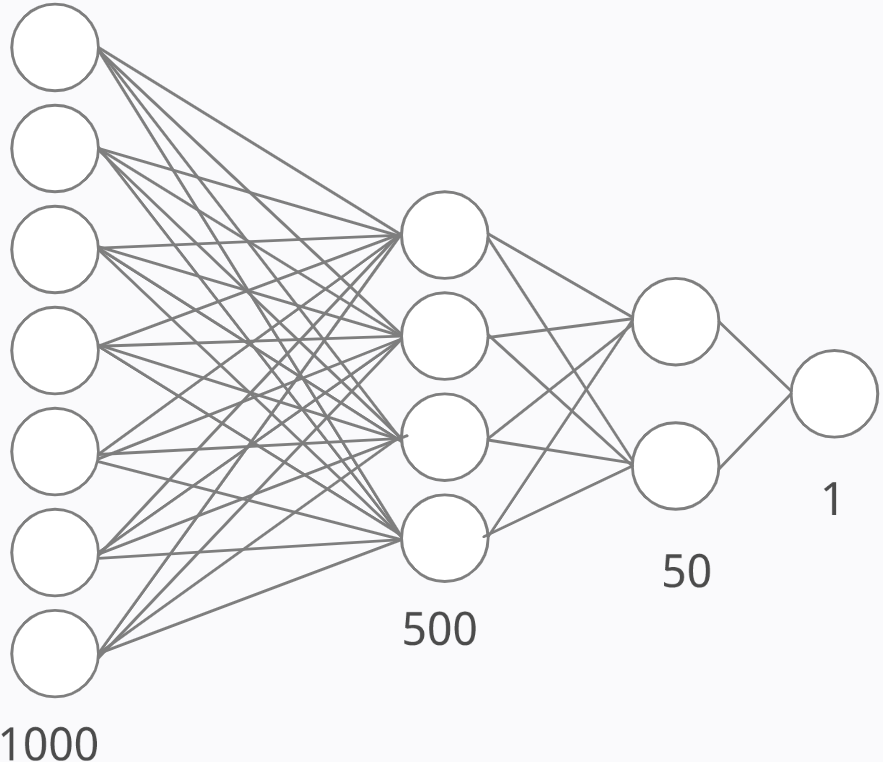
\includegraphics [scale=0.5] {img/model.png}
  \caption{Конечная схема спроектированной модели нейронной сети} 
  \label{fig:4}  
\end{figure}


\cite{18,21}.